%%%%%%%%%%%%%%%%%%%%%%%%%%%%%%%%%%%%%%%%%%%%%%%%%%%%
\section{Algorithm}

\subsection{Method Overview}

Apriori-Window is an exact enumeration algorithm that applies the
anti-monotonicity of Apriori~\cite{agrawal1994fast} to local frequency
evaluation in a sliding window.
The input is an event stream, window width $W$, threshold $\theta$,
and scan frequency $\Delta$; the output is the enumeration of all
dense patterns $X$ and their dense interval sets $\mathrm{DI}(X)$.

The algorithm starts from itemset size $k = 1$,
generates size-$(k{+}1)$ candidates from the dense pattern set $L_k$,
and computes dense intervals for each candidate iteratively.
For each itemset $X$, dense interval computation slides a window
$[l, l{+}W]$ from left to right while counting occurrences of $X$.
Scan Stride Skipping dynamically adjusts the slide width to skip
unnecessary scans and reduce computational cost.
Apriori Interval Pruning further narrows the search space using
the anti-monotonicity of support.

Scans are triggered every $\Delta$ seconds, resuming from the
endpoint of the previous scan to cover newly arrived events.
Smaller $\Delta$ improves real-time responsiveness; larger $\Delta$
reduces the number of scans and computational cost through the
benefit of Scan Stride Skipping.

Algorithm~\ref{alg:aw} presents the full procedure.
$\mathrm{Scan}$ is the monotone scan with Scan Stride Skipping,
and the candidate scan range $R_X$ is computed by Apriori Interval Pruning.

\begin{algorithm}[t]
\caption{Apriori-Window (single scan)}\label{alg:aw}
\begin{algorithmic}[1]
\Require $\mathit{occ}$: item $\to$ sorted timestamp list map; $W$; $\theta$
\Ensure $F$: pattern $\to$ dense interval set map
\State $F \leftarrow \emptyset$; $L_1 \leftarrow \emptyset$
\For{$x \in \mathrm{sorted}(\mathrm{keys}(\mathit{occ}))$}
  \State $\mathrm{DI}(x) \leftarrow \mathrm{Scan}(\mathit{occ}(x),\, W,\, \theta,\, \text{full range})$
  \If{$\mathrm{DI}(x) \neq \emptyset$}
    \State $F[\{x\}] \leftarrow \mathrm{DI}(x)$; $L_1 \leftarrow L_1 \cup \{\{x\}\}$
  \EndIf
\EndFor
\State $k \leftarrow 2$; $L_p \leftarrow L_1$
\While{$L_p \neq \emptyset$}
  \State $C_k \leftarrow \mathrm{AprioriJoin}(L_p)$
  \State $L_k \leftarrow \emptyset$
  \For{$X \in C_k$}
    \State $\mathit{occ}(X) \leftarrow \bigcap_{x \in X} \mathit{occ}(x)$
    \If{$\mathit{occ}(X) = \emptyset$} \textbf{continue} \EndIf
    \State $R_X \leftarrow \mathrm{cand}(X)$
    \If{$R_X = \emptyset$} \textbf{continue} \EndIf
    \State $\mathrm{DI}(X) \leftarrow \mathrm{Scan}(\mathit{occ}(X),\, W,\, \theta,\, R_X)$
    \If{$\mathrm{DI}(X) \neq \emptyset$}
      \State $F[X] \leftarrow \mathrm{DI}(X)$; $L_k \leftarrow L_k \cup \{X\}$
    \EndIf
  \EndFor
  \State $L_p \leftarrow L_k$; $k \leftarrow k + 1$
\EndWhile
\State \Return $F$
\end{algorithmic}
\end{algorithm}

\subsection{Scan Stride Skipping}

Na\"ively incrementing $l$ by one each step is inefficient.
Instead, intervals where density or non-density can be determined
without scanning are skipped.

For a fixed itemset $X$, let $\mathit{occ}(X)$ be the sorted list of
timestamps at which $X$ occurs.
Let $c = \mathrm{sup}(X, l, W)$ be the number of occurrences of $X$
in window $[l, l{+}W]$.
The left endpoint $l$ is updated via a two-branch stride according
to whether $c \geq \theta$ or $c < \theta$ (Fig.~\ref{fig:scan_stride}).

\textbf{Dense phase} ($c \geq \theta$):
Let $i_{\mathrm{start}}$ be the index of the first occurrence within the window.
Sliding the window right, even if the surplus $c - \theta$ occurrences
leave the window, the count remains at or above the threshold.
Therefore, $[l,\, \mathit{occ}(X)[i_{\mathrm{start}} + c - \theta] + W]$ is
output as a dense interval, and $l$ is updated as:
\begin{equation}\label{eq:stride_dense}
  l \leftarrow \mathit{occ}(X)[i_{\mathrm{start}} + c - \theta] + 1.
\end{equation}

\textbf{Non-dense phase} ($c < \theta$):
Let $i_{\mathrm{end}}$ be the index of the first occurrence after the window.
Since $c < \theta$, the next potentially dense left endpoint requires
$\theta - c$ additional occurrences to enter the window.
Therefore, $l$ jumps as:
\begin{equation}\label{eq:stride_sparse}
  l \leftarrow \mathit{occ}(X)[i_{\mathrm{end}} + (\theta - c) - 1] - W.
\end{equation}

The validity of both phases is established in Appendix~B
(Lemma~\ref{lem:stride_dense} and Lemma~\ref{lem:stride_sparse}).

\begin{figure}[t]
\centering
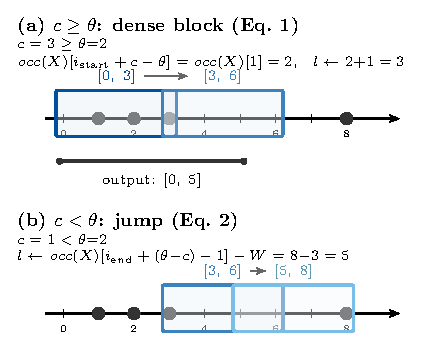
\includegraphics[width=\columnwidth]{scan_stride.pdf}
\caption{Scan Stride Skipping
  (Eqs.~\eqref{eq:stride_dense},~\eqref{eq:stride_sparse}).}
\label{fig:scan_stride}
\end{figure}

\subsection{Apriori Interval Pruning}

The anti-monotonicity of classical Apriori~\cite{agrawal1994fast}
states that every subset of a frequent itemset is also frequent;
equivalently, if any subset is infrequent, its supersets are infrequent.
We apply this property \textit{per interval}.
Since $Y \subseteq X$ implies that every occurrence of $X$ is also an
occurrence of $Y$, for any window $[l, l+W]$:
\[
  \mathrm{sup}(X, l, W) \leq \mathrm{sup}(Y, l, W)
\]
(Lemma~\ref{lem:apriori}, Appendix~C).
Hence if $[l, l+W]$ is not a dense interval for $Y$, it cannot be
one for $X$ either.
For a size-$k$ candidate $X$, the left endpoints $l$ that can be dense
are therefore restricted to the intersection of the dense start-point
sets of all $(k{-}1)$-subsets:
\begin{equation}\label{eq:cand}
  R_X = \bigcap_{Y \subsetneq X,\, |Y|=k-1} \mathcal{T}_\theta(Y),
\end{equation}
where $\mathcal{T}_\theta(Y)$ is the set of left endpoints for which $Y$
is dense.
Any $l \notin R_X$ can safely be skipped, substantially reducing
the scan range.

\subsection{$\Delta$-Step Streaming}

In the target deployment, events arrive continuously from a
sensor stream or autonomous agent log and are appended to a database.
The system triggers a scan every $\Delta$ seconds.

Each scan step proceeds as follows:

\begin{enumerate}
  \item When the $\Delta$-second interval has elapsed (current time $s$),
        retrieve the buffer $[s - W + 1,\; s + \Delta)$, retaining the
        $W{-}1$ most recent events from the previous step to
        prevent boundary loss.
  \item Run the monotone scan with Scan Stride Skipping and
        Apriori Interval Pruning over this buffer, resuming
        from the scan endpoint of the previous step.
  \item Emit all intervals $(X, [l_s, l_e])$ with $l_e + W \leq s$
        not yet output: these are \textbf{confirmed} and will not
        change as future events arrive.
  \item Wait for the next $\Delta$ seconds and repeat.
\end{enumerate}
